\newpage % Start models on a new page
\section{Models}
\subsection{Modeling and Solving of Problem 1}

\subsubsection{Calculation of each scheme}
\paragraph{Scheme a: Only Space Elevator System}
\vspace{0.3em}
太空电梯系统由三个银河港组成，每个银河港每年可运输17.9万吨货物，$P_{SES} = 3 \times 179000 = 537000\ \mathrm{kg/year}$。
根据国际太空电梯协会（ISEC）的预测，太空电梯的运营成本可降至$C_{SES} = \$100/\mathrm{kg}$，这包含了电力消耗、维修及折旧等费用。
因此，仅使用太空电梯系统的时间为
\[T=\frac{M}{P_{SES}}\]
Total cost of the mission为
\[C_{total} = C_{SES} \times M \]
计算得出：仅使用太空电梯系统需要约186.22年，总成本约10万亿美元。

\paragraph{Scheme b: Only Rocket Launches}
\vspace{0.3em}
利用现有的十个发射场进行高频发射，每个火箭发射可携带$P_{launch} = 100000kg$的有效载荷，
单发火箭的成本为$C_{launch} = \$500/\mathrm{kg}$。
若设定目标工期为40年，则每年需要发射的火箭次数为
\[x = \frac{M}{P_{launch} \times T} \]
Total cost of the mission为
\[C_{total} = C_{launch} \times M \]
计算得出：若仅使用火箭发射且在40年完成，总成本约50万亿美元，但每年需要发射25000次火箭，日均发射约68次，
单个发射场在一天内需要发射约7次，远超当前全球发射能力，在工程上极其困难。

\paragraph{Scheme c: Combined Space Elevator and Rocket Launches}
\vspace{0.3em}
综合考虑太空电梯系统和火箭发射两种方法时，这是一个多目标优化问题，目标是最小化任务完成时间$T$和总成本$C_{total}$。
通过调整火箭发射次数$x$来达到两种方法的不同组合，从中找到时间和成本之间的平衡点。
%为刻画混合航天运输系统中任务时间与总成本之间的权衡关系，本文构建了一种混合运载能力权衡优化模型（HCTO-PM），并通过显式 Pareto 前沿进行决策分析。
To analyze the trade-off between mission completion time and total cost in a hybrid space transportation system,
a Hybrid Capacity Trade-off Optimization model with explicit Pareto Mapping (HCTO-PM) is developed.
该模型采用单参数控制的并行运输系统结构，决策变量$x$表示火箭的年发射次数，目标函数包括任务完成时间$T$和总成本$C_{total}$。
任务完成时间$T$由以下公式给出：
\[T = \frac{M}{P_{SES} + P_{launch} \times x} \]
总成本$C_{total}$由以下公式给出：
\[C_{\mathrm{total}}(x)=C_{SES}\cdot P_{SES}\cdot\frac{M}{P_{SES}+xP_{launch}}+C_{launch}\cdot P_{launch}\cdot x\]
Multi-Objective Formulation:
The model simultaneously considers the following two conflicting optimization objectives.
\[\begin{cases}
\min T(x)=\frac{M}{P_{\mathrm{SES}}+xP_{\mathrm{launch}}} \\
\min C(x)=C_{\mathrm{total}}(x) & 
\end{cases}\]
Without the assumption of explicit preference weights, this problem does not pursue a single optimal solution, 
but instead constructs a Pareto optimal solution set to characterize the efficiency boundary in the feasible decision space.
Since the model contains only one continuous decision variable, this paper uses the parameter sweep method to
perform high-resolution sampling of the feasible interval of $x$.
计算对应的时间–成本目标值，并通过非支配关系筛选得到 Pareto 前沿。
%\begin{figure}[htbp]
%    \centering
%    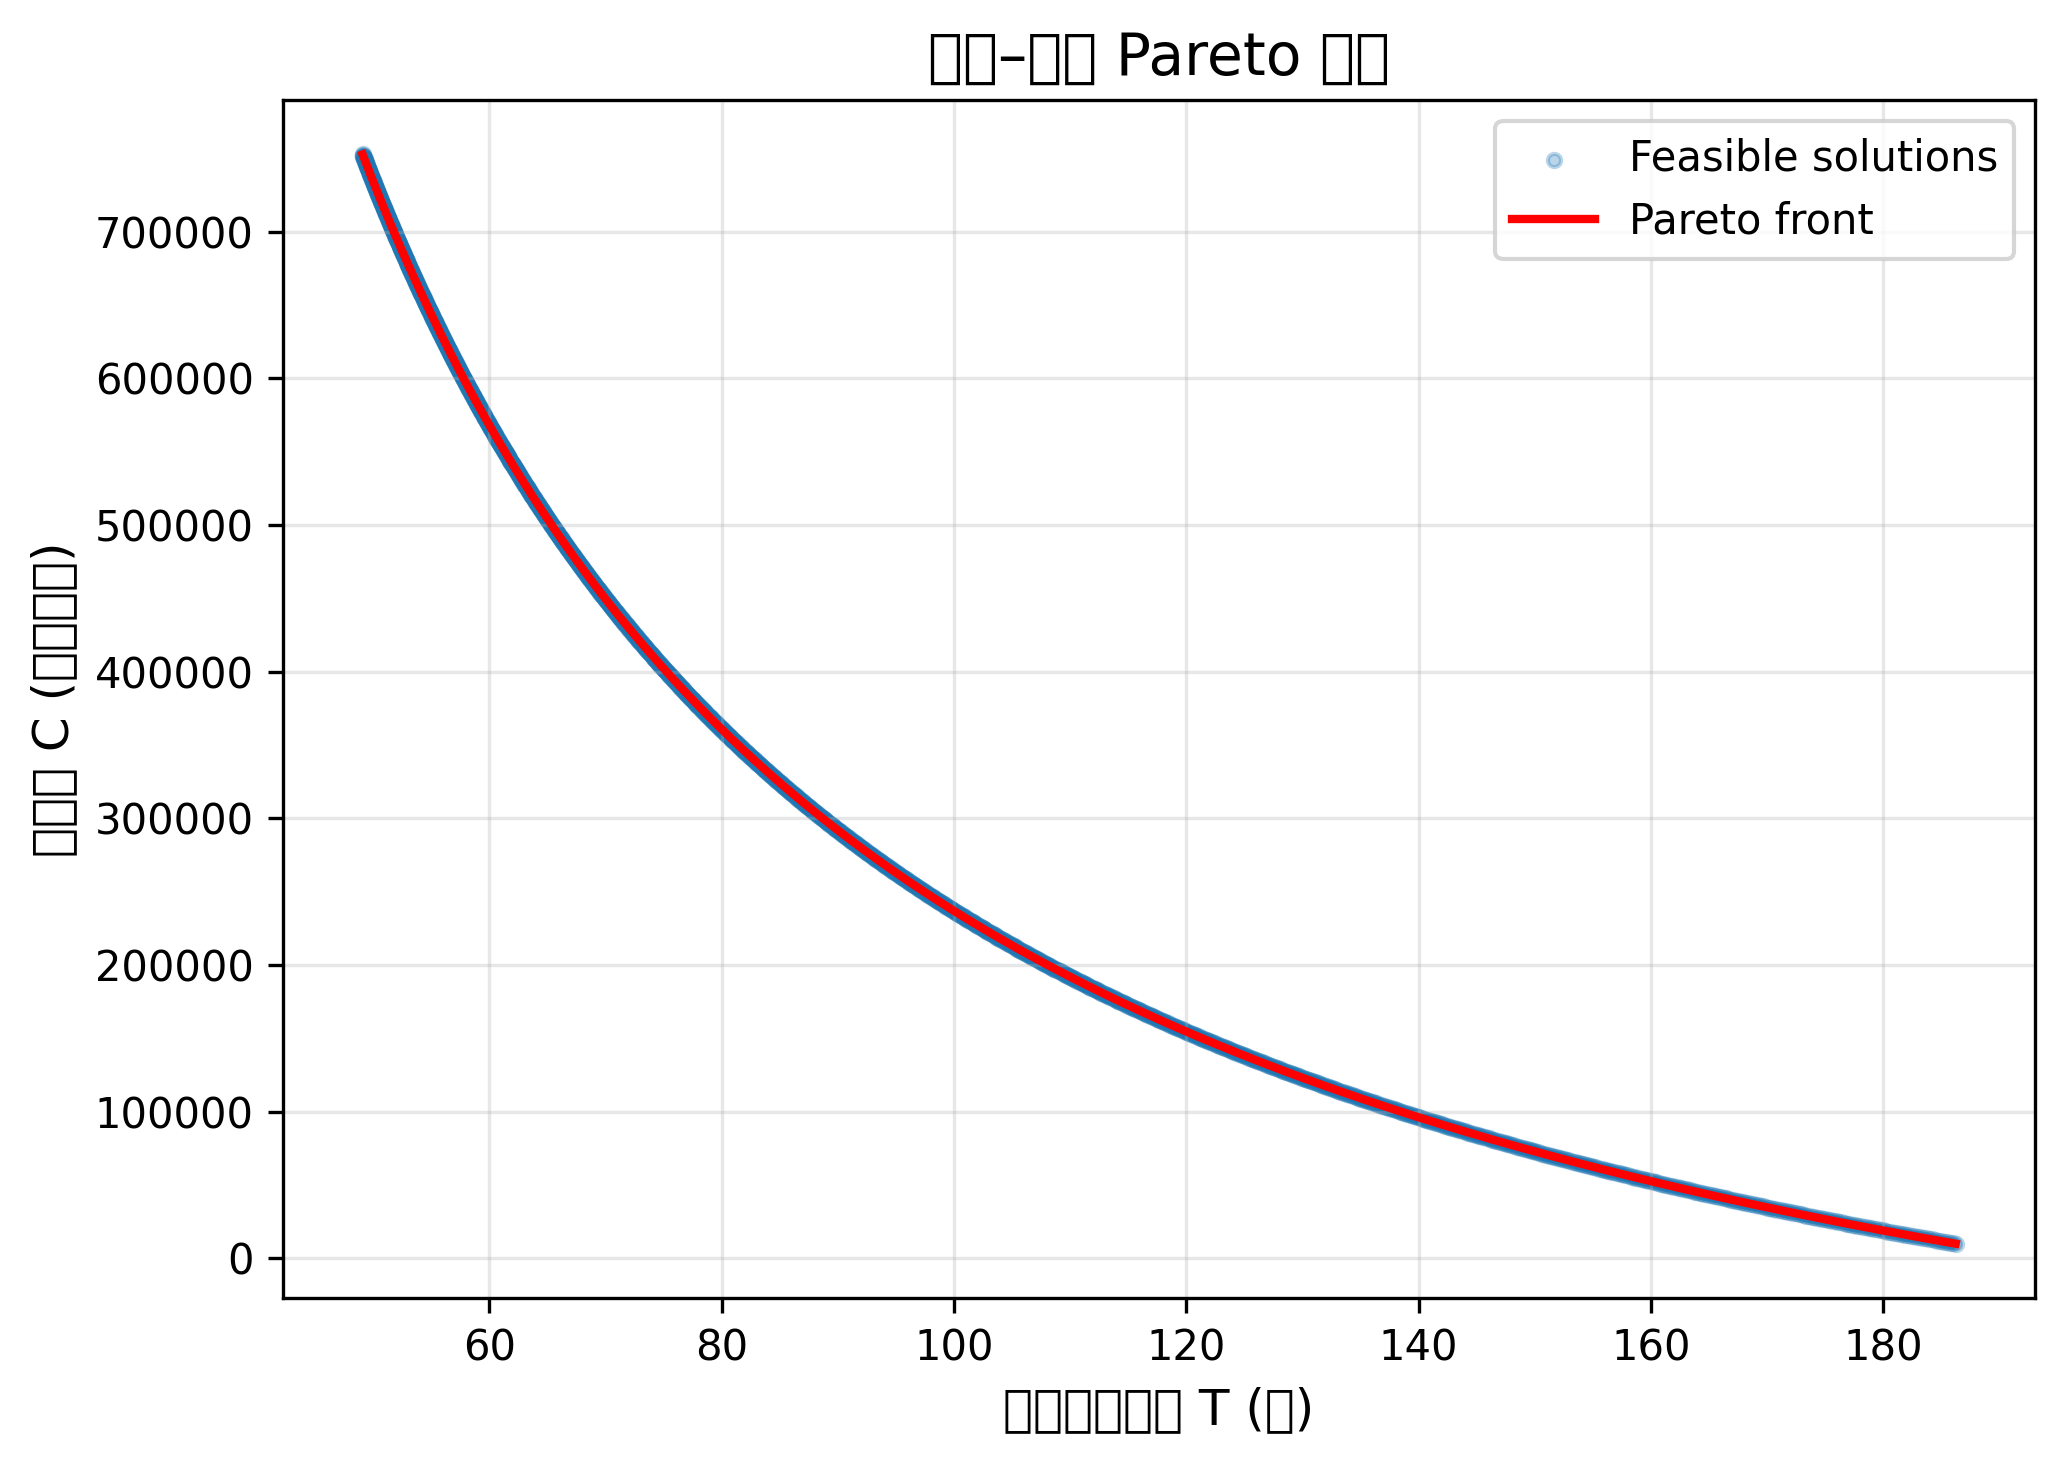
\includegraphics[width=0.65\textwidth]{figures/pareto_scan.png}
%    \caption{时间–成本多目标优化问题的 Pareto 前沿}
%    \label{fig:pareto_scan}
%\end{figure}
%图~\ref{fig:pareto_scan}展示了时间–成本多目标优化问题的 Pareto 前沿。
从中选出部分关键解得到如下表格：
\begin{table}[htbp]
\centering
\caption{Trade-off Results under Different Rocket Launch Frequencies}
\label{tab:tradeoff_results}
\renewcommand{\arraystretch}{1.3}
\begin{tabular}{c c c}
\toprule
\textbf{Rocket Launches} $x$ (\textbf{times/year}) 
& \textbf{Completion Time} $T$ (\textbf{years}) 
& \textbf{Total Cost} $C$ (\textbf{million USD}) \\
\midrule
2{,}496  & 109.72 & 193{,}110.40 \\
4{,}997 & 77.72 & 378{,}986.12 \\
7{,}499 &49.09 & 752{,}636.23 \\
\bottomrule
\end{tabular}
\end{table}
根据不同的决策偏好可以从中选择适当的解决方案。
贴图

\subsubsection{Improvement of scheme c}
\paragraph{Rocket Iteration: Transportation cost iteration}
\vspace{0.3em}
理论基础:
在分析每 100kg 有效载荷的运输成本演变时，必须引入工业经济学中的核心概念——学习曲线模型（Learning Curve Model），
即莱特定律（Wright's Law）。该定律由 T.P. Wright 最早于 1936 年在航空制造领域提出，其核心论点表明：单位产品的生产成本
并不是随机波动的，而是随着累计产量的增加呈现出可预测的幂律下降趋势。在商业航天领域，这一效应被进一步修正为受“规模经济”与“复用频率”双重驱动的成本迭代机制。
在构建长周期的航天运输成本演变模型时，若仅采用单一的指数衰减模型，容易忽略物理化学层面的硬性约束。因此，本研究引入双因子成本结构（Dual-Factor Cost Structure），
将单次发射的单位质量成本  解构为两个性质迥异的组成部分：受工业学习曲线影响的箭体制造与运营成本$C_{body}$，以及受化学工业定价影响的相对刚性的燃料（推进剂）成本 $C_{fuel}$ 。
根据工业经济学中的莱特定律（Wright's Law），箭体制造与发射运营成本具有显著的“干中学”（Learning by Doing）特征，即随着累计发射量和复用次数的增加，该部分成本呈现幂律下降。
然而，燃料成本主要取决于液氧、甲烷或煤油的工业大宗商品价格，其波动受宏观能源市场影响，难以通过航天产业自身的规模效应实现数量级下降。因此，成本动力学方程应表达为：
\[C_{launch}=C_{man}(n)+C_{fuel}=C_1\cdot n^{-b}+C_{fixed}\]
其中，$n$ 为累计产出量，$b$ 为学习指数，而 $C_{fixed}$ 代表了由化学能密度决定的热力学成本底限。这一模型的引入，揭示了航天运输成本下降虽然在初期极其迅速，但在远期将逼近一个由物理极限决定的渐进值。
通过历史数据回溯可以发现，航天运输成本的结构正经历着从“硬件主导”向“能源主导”的范式转移。在传统航天飞机时代，每公斤约 54,500 美元的发射成本中，推进剂成本占比微乎其微（不足 0.1\%），绝大部分开支源于
一次性的硬件损耗与高昂的地面维护。此时，莱特定律对整体成本的削减作用极为显著。随着 SpaceX 猎鹰 9 号（Falcon 9）及星舰（Starship）架构的出现，高频复用技术彻底改变了这一比例。根据 ARK Invest 与
SpaceX 公开财务数据的交叉验证，猎鹰 9 号的燃料成本约为 20-30 万美元，仅占单次发射边际成本的极小比例，但在完全复用的星舰架构预期中，随着硬件均摊成本的急剧下降，燃料成本的占比将大幅提升。根据埃隆·马斯克
的工程预期，未来星舰的单次发射成本中，推进剂费用将成为主要的边际支出项。这表明，虽然制造成本可以通过 30\%-35\% 的高学习率（Learning Rate）快速摊薄，但燃料成本将构成一条不可逾越的水平渐近线（Horizontal Asymptote）。

参数设定:
为了构建适用于年度预测的数学模型，我们将基于“产量”的莱特定律映射为基于“时间”的年度衰减函数，并设定燃料成本为常量约束。假设全球航天发射频率维持当前的指数增长趋势，制造成本部分的年均优化效率将维持高位。
基于现有技术路径的分析，本模型设定如下核心参数：
- 制造成本衰减率：考虑到规模效应与复用技术的成熟，设定箭体制造与运营部分的年均衰减系数$\alpha$为 5\%。
- 燃料成本刚性：设定每 100kg 有效载荷分摊的燃料成本为常数$C_{fuel}$，作为成本演化的收敛极限。
综合考量，未来的单位运输成本将不再是无限趋近于零，而是沿着一条指数曲线逼近燃料成本底线。这种处理方式平抑了纯数学模型在远期预测中的失真风险，符合大规模物流网络的物理现实。

模型构建:
基于上述双因子分析，本研究建立每 100kg 货物运输成本$C_{launch}(t)$随时间$t$演变的最终迭代公式：
设$t$为年份(以模型起始年为$t = 0$)，$C_{launch}(t)$由可变动的制造部分$C_{man}(t)$和固定的燃料部分$C_{fuel}$，则有：
\[C_{launch}(t)=C_{man_0}\times(1-\alpha)^t+C_{fuel}\]
带入参数得：
\[C_{launch}(t)=(C_{total_0}-C_{fuel})\times(0.95)^t+C_{fuel}\]
该公式清晰地描述了成本下降的两个阶段：在近期（$t$较小时），由$(1 - \alpha)^t$主导，体现为成本的快速下降，符合摩尔定律般的指数特征；在远期（$t$趋于无穷大时）， $C_{launch}(t)$渐近收敛于 $C_{fuel}$，体现了能源价格对太空物流经济性的最终约束。

\paragraph{A new strategy based on the iterative models}
\vspace{0.3em}
基于上述迭代模型，我们提出了一种新的混合运输策略，以进一步优化运输成本与时间的权衡。在HCTO-PM模型的基础上，结合时间变量$t$引入动态成本调整机制来反映火箭发射成本随时间的演变，得到
Multi-Year Hybrid Capacity Trade-off Optimization with Pareto Mapping (MY-HCTO-PM)模型。该模型下的决策变量$x$不在是单一维度，而是会随着时间$t$动态调整的函数$x(t)$，以反映不同年份的发射频率选择。
优化目标函数同样包括任务完成时间$T$和总成本$C_{total}$，计算公式为
\[P_{SES}T+P_{launch}\cdot\sum_{t=0}^{T}x_{(t)} = M\]
\[C_{total}=C_{SES}\cdot P_{SES}\cdot T+\sum_{t=0}^{T}C_{launch}(t)\cdot x_{(t)}\cdot P_{launch}\]
对每个可行$T$, 求出用火箭发射的总运输质量后按年份倒序分配（从最后一年开始发射），以利用制造成本衰减优势。得到一组$(T,C)$ 数据点，即帕累托前沿。
为便于决策，定义三类代表性解：
- 均衡解（Balanced）：使用归一化后的时间和成本计算每个可行点到理想点 $(T_{min}, C_{min})$ 的欧氏距离，距离最小者即为均衡解
- 激进解（Faster）：均衡解向左偏移一定比例（减少总工期，允许成本增加）
- 经济解（Cheaper）：均衡解向右偏移一定比例（延长总工期以降低成本）
该方法保证了三类方案均落在最优折中区间内，可直观展示工期与成本之间的权衡关系。
% 贴图


\subsubsection{Conclusions of Problem}
太空电梯和传统火箭的组合更有利于实现高效且经济的太空运输。通过调整火箭发射频率，可以在任务完成时间和总成本之间找到最佳平衡点。
引入火箭运输成本的时间迭代模型后，提出了一种新的混合运输策略，进一步优化了运输方案。该策略通过动态调整火箭发射频率，利用制造成本的衰减优势，实现了更低的总成本和更短的任务时间。
基于MY-HCTO-PM模型，决策者可以根据不同的偏好选择均衡、激进或经济的运输方案，从而更好地满足实际需求。


\subsection{Modeling and Solving of Problem 2}
\subsubsection{Problem Analysis}


\subsubsection{Model Preparation}


\subsubsection{Model Construction}



\subsubsection{Model Solution}
